%
% uaThesis example (for a thesis written in Portuguese)
%
% the complete list of options and commands can be found in uaThesis.sty
%

\documentclass[11pt,twoside,a4paper]{report}
\usepackage[utf8]{inputenc}
\usepackage[DETI,newLogo]{uaThesis}

\def\ThesisYear{2023}

% optional packages
\usepackage[english]{babel}
\usepackage{hyperref}
\usepackage{amsmath}
\usepackage{amssymb}
\usepackage{xspace}% used by \sigla
\usepackage{listings}
\usepackage{multicol}
\usepackage{graphicx}
\usepackage{acronym}
\usepackage[acronym]{glossaries}

% optional (comment to use default)s
%   depth of the table of contents
%     1 ... chapther and sections
%     2 ... chapters, sections, and subsections
%     3 ... chapters, sections, subsections, and subsubsections
\setcounter{tocdepth}{3}

% optional (comment to used default)
%   horizontal line to separate floats (figures and tables) from text
\def\topfigrule{\kern 7.8pt \hrule width\textwidth\kern -8.2pt\relax}
\def\dblfigrule{\kern 7.8pt \hrule width\textwidth\kern -8.2pt\relax}
\def\botfigrule{\kern -7.8pt \hrule width\textwidth\kern 8.2pt\relax}

% custom macros (could also be defined using \newcommand)
\def\I{\mathtt{i}}         % one possible way to represent $\sqrt{-1}$
\def\Exp#1{e^{2\pi\I #1}}  % argument inside braces, i.e., "{}"
\def\EXP#1.{e^{2\pi\I #1}} % argument finishes when a full stop is encountered, i.e., "."
\def\sigla{\LaTeX\xspace}  % use as "blabla \sigla blabla (no need to do "blabla \sigla\ blabla"

\def\AddVMargin#1{\setbox0=\hbox{#1}%
                  \dimen0=\ht0\advance\dimen0 by 2pt\ht0=\dimen0%
                  \dimen0=\dp0\advance\dimen0 by 2pt\dp0=\dimen0%
                  \box0}   % add extra vertical space above and below the argument (#1)
\def\Header#1#2{\setbox1=\hbox{#1}\setbox2=\hbox{#2}%
           \ifdim\wd1>\wd2\dimen0=\wd1\else\dimen0=\wd2\fi%
           \AddVMargin{\parbox{\dimen0}{\centering #1\\#2}}} % put #1 on top #2


\makeglossaries

%
% Acronyms
%
\acrodef{ua}[UA]{University of Aveiro}
\acrodef{iris}[IRIS-Lab]{Intelligent Robotics and Systems Laboratory}
\acrodef{p2p}[P2P]{Peer to Peer}
\acrodef{ros}[ROS]{Robot Operating System}
\acrodef{rtt}[RTT]{Round Trip Time}
\acrodef{ddos}[DDOS]{Distributed Denial Of Service}
\acrodef{oor}[OOR]{Open Overlay Router}
\acrodef{nat}[NAT]{Network Address Translator}
\acrodef{sa}[SA]{Security Association}
\acrodefplural{sa}[SAs]{Security Associations}
\acrodef{ah}[AH]{Authentication Header}
\acrodef{esp}[ESP]{Encapsulating Security Payload}
\acrodef{spi}[SPI]{Security Parameter Index}
\acrodef{ike}[IKE]{Internet Key Exchange}
\acrodef{icv}[ICV]{Integrity Check Value}
\acrodef{ssl}[SSL]{Secure Sockets Layer}
\acrodef{DERP}[DERP]{Designated Encrypted Relay for Packets}
\acrodef{stun}[STUN]{Session Traversal Utilities for NAT}
\acrodef{edm}[EDM]{Endpoint-Dependent Mapping}
\acrodef{eim}[EIM]{Endpoint-Independent Mapping}
\acrodef{http}[HTTP]{Hyper-Text Transfer Protocol}
\acrodef{vpn}[VPN]{Virtual Private Network}
\acrodefplural{vpn}[VPNs]{Virtual Private Networks}
\acrodef{ip}[IP]{Internet Protocol}
\acrodef{ap}[AP]{Access Point}
\acrodef{vlan}[VLAN]{Virtual Local Area Network}
\acrodef{ttl}[TTL]{Time To Live}
\acrodef{ssh}[SSH]{Secure Shell}
\acrodef{cli}[CLI]{Command Line Interface}
\acrodef{uri}[URI]{Uniform Resource Identifier}
\acrodef{url}[URL]{Uniform Resource Locator}
\acrodef{udp}[UDP]{User Datagram Protocol}
\acrodef{tcp}[TCP]{Transmission Control Protocol}
\acrodef{json}[JSON]{Java-Script Object Notation}
\acrodef{cdn}[CDN]{Content Distribution Network}
\acrodefplural{cdn}[CDNs]{Content Distribution Networks}
\acrodef{sdwan}[SD-WAN]{Software-Defined WAN}
\acrodef{ron}[RON]{Resilient Overlay Networks}
\acrodef{iot}[IoT]{Internet of Things}
\acrodef{https}[HTTPS]{Hyper-Text Transfer Protocol Secure}
\acrodef{le}[LE]{Let's Encrypt}
\acrodef{fqdn}[FQDN]{Fully Qualified Domain Name}
\acrodef{acl}[ACL]{Access Control List}
\acrodefplural{acl}[ACLs]{Access Control Lists}

\begin{document}


%
% Cover page (use only one of the first two \TitlePage)
%

%
% Initial thesis pages
%

\TitlePage
  \HEADER{\BAR\FIG{\begin{minipage}{50mm} % no more than 120mm
          ``An idiot admires complexity, a genius admires simplicity.''
           \begin{flushright}
            --- Terry A. Davis
           \end{flushright}
          \end{minipage}}}
         {\ThesisYear}
  \TITLE{Vasco Regal Sousa}
        {Multiple Client WireGuard Based Private and Secure Overlay Network}
\EndTitlePage
\titlepage\ \endtitlepage % empty page

\TitlePage
  \vspace*{55mm}
  \TEXT{\textbf{o j\'uri~/~the jury\newline}}
       {}
  \TEXT{presidente~/~president}
       {\textbf{ABC}\newline {\small
        Professor Catedr\'atico da Universidade de Aveiro (por delega\c c\~ao da Reitora da
        Universidade de Aveiro)}}
  \vspace*{5mm}
  \TEXT{vogais~/~examiners committee}
       {\textbf{DEF}\newline {\small
        Professor Catedr\'atico da Universidade de Aveiro (orientador)}}
  \vspace*{5mm}
  \TEXT{}
       {\textbf{GHI}\newline {\small
        Professor associado da Universidade J (co-orientador)}}
  \vspace*{5mm}
  \TEXT{}
       {\textbf{KLM}\newline {\small
        Professor Catedr\'atico da Universidade N}}
\EndTitlePage
\titlepage\ \endtitlepage % empty page

\TitlePage
  \vspace*{55mm}
  \TEXT{\textbf{agradecimentos~/\newline acknowledgements}}
       {\'Agradecimento especial aos meus gatos}
  \TEXT{}
       {Desejo tamb\'em pedir desculpa a todos que tiveram de suportar o meu desinteresse pelas
        tarefas mundanas do dia-a-dia}
\EndTitlePage
\titlepage\ \endtitlepage % empty page


\TitlePage
  \vspace*{55mm}
  \TEXT{\textbf{Abstract}}
       {An overlay network is a group of computational nodes that communicate with each other through a virtual or logic channel, built on top of another network. Although there are already numerous services and protocols implementing this mechanic, scalability and administration agility are among the most desired characteristics of such a network topology. Hence, this document presents a centralized solution for the creation and control of secure overlay networks for multiple nodes - from client management to operation auditing, based on WireGuard, an open-source protocol for encrypted communication. In the University of Aveiro, namely the autonomous robot ecosystem residing in the IRIS lab, supporting such a networking architecture would prove to be particularly interesting, both for development and solution deployment.}
\EndTitlePage
\titlepage\ \endtitlepage % empty page


%
% Tables of contents, of figures, ...
%
\pagenumbering{roman}
\tableofcontents

\cleardoublepage
\listoffigures

\cleardoublepage
\listoftables

\cleardoublepage
% \printglossary[type=\acronymtype]

% The chapters (usually written using the isolatin font encoding ...)

\cleardoublepage
\pagenumbering{arabic}
\chapter{Introduction}

\section{Motivation}

Network security has become a topic of growing interest in any information system. Companies strive to ensure their communications follow principles of integrity and confidentiality while minimizing attack vectors that could compromise services and data. With such goals in mind, network topologies are subjected to traffic constraints and security mechanisms to protect their systems.

Such is the case in the \ac{ua}, where the network, although covering most of the campus' area, enforces several constraining mechanisms that prevent, for example, the establishment of direct \ac{p2p} connections between two clients.

The \ac{iris} is a research unit operating in \ac{ua}'s premises which develops projects using autonomous mobile robots, capable of communicating through a wireless network. Currently, the robots are confined to the laboratory's internal network, since, as mentioned above, \ac{ua}'s highly restrictive network prevents the robots from communicating directly using \ac{ua}'s network, also refered to as \textbf{eduroam}.

Overcoming these limitations would be extremly valuable for \ac{iris}'s developments. In fact, allowing robots to communicate directly in a \ac{p2p} communication would not only enable solutions across multiple buildings but also aid researchers during development, as they would be able to interact with the robots directly through their personal machines.

\section{Objectives}

This dissertation aims to implement a private overlay network manager to be used exclusively by \ac{ua}'s clients. The concept of an overlay network entails the creation of a communication layer built on top of an already existing network.

In the \ac{iris} scenario, the management platform should provide operations to achieve a secure, private communication between a group of robots connected to \ac{ua}'s network, regardless of their physical location within the campus. Moreover, the authentication and connection to a desired overlay network by the robots must be a seamless operation, requiring little to no manual configuration.

To reinforce the privacy and confidentiality, this solution should be hosted entirely within \ac{ua}'s premises, preferably using open source tools.

Therefore, the objectives for this dissertation can be summarized as (i) enabling secure \ac{p2p} communications between clients connected to \ac{ua}'s network, (ii) automation of client deployment, authentication and configuration mechanisms, creating an abstraction layer for the usual robot operations and (iii) ensure communication overhead is suitable for \ac{iris}'s projects requirements.

\section{Document Structure}

This document presents an implementation of such an overlay network manager. Hence, it is structured in two main chapters, the state of the art and the methodology. The former describes an exploration of the background and current state of the art, providing an analysis not only of potential tools, protocols, and frameworks suitable for the scope of the dissertation but also of published research conducted covering similar topics and scenarios. The latter establishes the work methodology to be taken for the development and results gathering process.


\cleardoublepage

\chapter{Background and State of the Art}
\label{chapter:sota}

\begin{minipage}{80mm}
     \centering % no more than 120mm
     ``O caos é uma ordem por decifrar''
          \begin{flushright}
          --- José Saramago
          \end{flushright}
     \end{minipage}


\section{Overlay Networks}
\label{sec:on}

In the last few decades, the Internet has been subjected to an exponential growth, both in the number of users and connected devices. To answer the increasing demand and support aspects such as mobility and scalibility, Internet applications have diverged from classic distributed systems to more complex network topologies, creating an extremly heterogeneous environment. In such a non-patternized landscape, \ac{p2p} overlay networks have emerged as a topic of growing interest, as conducted research on the matter attempts to create networking solutions capable of addressing the adversities imposed by the modern day Internet. This section explores the fundamental principles of overlay networks and how its abstraction layer is able to produce a topology with the potential to bring a logical order to  the chaotic network architecture of the Internet.

By definition, an overlay network is a logical network implemented on top of the links of another, already established, underlay network ~\cite{livronet}. In other words, nodes (also called peers) in an overlay network (which also exist in the underlay network) implement its own application-defined routing and datagram processing behaviour. Hence, the Internet application running in the nodes is responsible for the creation and management of the \ac{p2p} logical links that form the overlay network. Figure \ref{fig:overlay} illustrates this concept.

\begin{figure}[h]
\centering
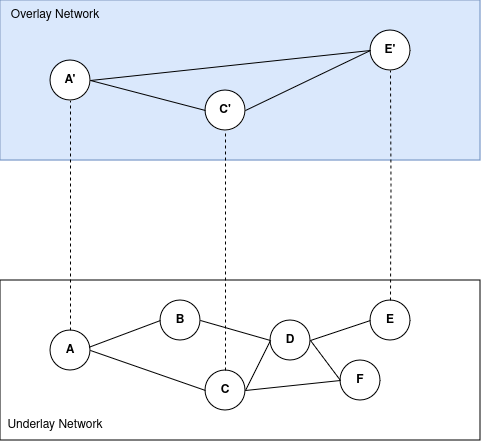
\includegraphics[width=0.5\textwidth]{overlays.png}
\caption{Concept of a very basic overlay network. Nodes A, C and E create logical links with each other, forming an overlay network}
\label{fig:overlay}
\end{figure}

Overlay networks can be used in applications to achieve numerous functionalities, such as finding alternate routes for unicast applications, explored by \ac{ron} ~\cite{ron}, which measures peers' average latencies in order to discover routes optimizing network end-to-end reliability and performance. This idea is also the principle behind \ac{sdwan} services, where forwarding rules are dynamically reconfigured and automated according to a set of defined policies, an emerging paradigm with prominent results ~\cite{9203058, 9492375}. Another common example of the use of overlay networks are object sharing applications such as BitTorrent, where the overlay network is formed by the nodes which possess parts of the desired file. When a peer wants to download a file, it establishes \ac{p2p} connections to the other overlay peers and retrieves the part of the data until the file is complete ~\cite{5482574}.

While decentralized by design, some topologies applying overlay concepts have a degree of centralization, generally serving information regarding active peers in the network. Although a central point can cause bottlenecks, on-demand peer information is able to make a system easier to scale and reconfigure. BitTorrent is an example of this, where a new peer queries a central server, called a tracker, retrieving the addresses and identification of the peers it should connect to. Such centralization can, however, be discarded by implementing a peer finding algorithm which relies solely on the other peers already in the network.

As the nodes in an overlay network are systems running Internet applications, they are generally capable of performing more computational demanding operations than simply forwarding traffic, which is the case when dealing with devices in the underlay network, like routers or switches. Routing traffic through a node allows any application-defined manipulation to be applied to the datagrams, namely cryptographic operations. This idea is explored in further sections, as it serves as the backbone in several encrypted \ac{p2p} communication protocols.

Summarizing, the use of overlay networks provides an efficient and reliable way to create a logical structure between a set of nodes residing in an otherwise unstructured topology. Additionally, as overlay nodes are essentially end systems, there's great leverage for applications to freely manipulate and route traffic. By relying on \ac{p2p} communications, overlay networks' decentralized nature provides a very scalable and reconfigurable design.

\section{Virtual Private Networks}

Public networks are built on infrastructure users generally have no control over. Public routers, relay nodes, servers and even physical links always carry the risk of traffic eavesdropping and tampering by untrusted entities. Therefore, to ensure the confidentiality, privacy and integrity of connections established through an insecure medium, data should be properly encrypted and authenticated. One such mechanism is the use of \acp{vpn}.

Conceptually, a \ac{vpn} is a virtual network that provides functionalities which secure the transmission of data between any two endpoints ~\cite{HARMENING2017843}. This section aims to analyze how \acp{vpn} architecures have evolved, from its inception to more recent paradigms, which follow overlay concepts discussed in Section \ref{sec:on}. Then, it presents an overview of notable \ac{vpn} providers and their respective pros, cons and suitability for the scope of this solution. This state of the art survey aims to pickup on similar works ~\cite{zuqueteseguranca, berger2006analysis}, while additionally reviewing emerging protocols.

\subsection{VPN architectures}

Traditional \ac{vpn} services operate under a hub-and-spoke architecture, a model composed by one or more \ac{vpn} Gateways - devices accepting incoming connections from client nodes and forwarding the traffic to their final destination. Hub-and-spoke architectures carry some well known bottlenecks ~\cite{ELHEDHLI20051615, o1998geographer}. First, it implies increased latency associated with the geographical distance between a client and the nearest hub. Also, regarding scalability and dynamic configuration, adding new clients to the network requires the distribution of its keys to all hubs.

\ac{vpn}s can be classified according to their topology in two main categories: client-to-site and site-to-site. A client-to-site \ac{vpn} is characterized by connections from a single user (client) to a private network (site), while site-to-site \ac{vpn}s offer a secured connection between two private networks. Thus, in site-to-site networks, users are not required to individually configure \ac{vpn} clients. The tunnel in this type of \ac{vpn} is made available to the entire network.

\subsection{VPNs on NAT Networks}

\ac{nat} is a networking mechanism responsible for translating \ac{ip} addresses in private networks into public addresses when packets sent from a private network are routed to the public Internet. In the context of \ac{vpn} communications, this process can prove to be a major constraint, not only due to \ac{nat}'s tampering of \ac{ip} packets' fields, namely destination and source addresses, which could potentially compromise its integrity in the eyes of a \ac{vpn} protocol, but also regarding the dynamically changing public \ac{ip} addresses which \ac{nat} decides to translate private addresses to.

In fact, it is very likely that devices on the internet reside in a network behind both \ac{nat} mechanisms and Firewall rules, with no open ports. Also, believing nodes will have a consistent static \ac{ip} is a very naive assumption, especially when considering mobile devices. NAT Traversal is a networking technique that enables the establishing and maintaining (by keeping \ac{nat} holes open) of \ac{p2p} connections between two peers, no matter what's standing between them, making communication possible without the need for firewall configurations or public-facing open ports. There's no one solution to achieve this functionality. In fact, there are various developments effectively implementing a NAT Traversal solution, such as ICE ~\cite{rfc8445} and STUN ~\cite{rfc8489}. Hence, each \ac{vpn} service can have its own way of supporting NAT Traversal. Each case is explored separately in its own subsection.


\section{VPN Providers}

\subsection{IPSec}

IPSec refers to an aggregation of layer 3 protocols that work together to create a security extension to the \ac{ip} protocol by adding packet encryption and authentication. Conceptually, IPSec presents two main dimensions: the protocol defining the transmitted packets' format, when security mechanisms are applied to them, and the protocol defining how parties in a communication negotiate encryption parameters.

Communication in an IPSec connection is managed according to \acp{sa}. A \ac{sa} is an unidirectional set of rules and parameters specifying the necessary information for secure communication to take place ~\cite{rfc4301}. Here, unidirectional means a \ac{sa} can only be associated with either inbound or outbound traffic, but never with both. Hence, an IPSec bidirectional association implies the establishment of two \acp{sa}: one for incoming packets and one for outgoing. \acp{sa} specify which security mechanism to use - either \ac{ah} or \ac{esp} - and are identified by a numeric value, the \ac{spi}. Although \ac{sa}s can be manually installed in routers, gateways or machines, it becomes impractical as more clients appear. \ac{ike} ~\cite{rfc7296} is a negotiation protocol that tackles the problems associated with manual \ac{sa} installation. In fact, \ac{ike} allows the negotiation of \ac{sa} pairs between any two machines through the use of asymmetric keys or shared secrets.

\subsubsection{Transport and Tunnel modes}

IPsec supports two distinct modes of functionality: transport and tunnel ~\cite{rfc4301}, which differ in the way traffic is dealt with and processed. In the context of \ac{vpn}s, tunnel mode presents the
most desirable characteristics. First, tunnel mode encapsulates the original \ac{ip} packet, allowing the use of private \ac{ip} addresses as source or destination. Tunnel mode creates the concept of an ``outer" and ``inner`` \ac{ip} header. The former contains the addresses of the IPSec peers, while the latter contains the real source and destination addresses. Moreover, this very same encapsulation adds confidentiality to the original addresses.

Transport mode requires fewer computational resources and, consequently, carries less protocol overhead. It does not, however, provide much security compared to tunnel mode, so, in the context of \ac{vpn}s, tunnel mode's total protection and confidentiality of the encapsulated \ac{ip} packet carry much more valuable functionalities.

\subsubsection{Authentication Header}

\ac{ah} is a protocol in the IPSec suite providing data origin validation and data integrity consisting in the generation of a checksum via a digest algorithm ~\cite{rfc4302}. Additionally, besides the actual message under integrity check, two other parameters are used under the \ac{ah} mechanism. First, to ensure the message was sent from a valid origin, \ac{ah} includes a secret shared key. Then, to ensure replay protection, it also includes a sequence number. This last feature is achieved with the sender incrementing a sequence integer whenever an outgoing message is processed.

\ac{ah}, as the name suggests, operates by attaching a header to the \ac{ip} packets, containing the message's \ac{spi}, its sequence number, and the \ac{icv} value. This last field is then verified by receivers, which calculate the packet's \ac{icv} on their end. The packet is only considered valid if there's a match between the sender and receiver's \ac{icv}.

Where this header is inserted depends on the mode in which IPSec is running. In transport mode, the \ac{ah} appears after the \ac{ip} header and before any next layer protocol or other IPSec headers. As for tunnel mode, the \ac{ah} is injected right after the outer \ac{ip} header.

To calculate the \ac{icv}, the \ac{ah} requires the value of the source and destination addresses, which raises an incompatibility when faced with networks operating with \ac{nat} mechanisms ~\cite{frankel2005guide}.

\subsubsection{Encapsulating Security Payload}

The \ac{esp} protocol also offers authentication, integrity and replay protection mechanisms. It differs from \ac{ah} by also providing encryption functionalities, where peers in a communication use a shared key for cryptographic operations. Analogous to the previous protocol, the \ac{esp}'s header location differs in different IPSec modes. In transport mode, the header is inserted right after the \ac{ip} header of the original packet. Also, in this mode, since the original \ac{ip} header is not encrypted, endpoint addresses are visible and might be exposed. As for tunnel mode, a new \ac{ip} header is created, followed by the \ac{esp} header.

Tunnel mode \ac{esp} is the most commonly used IPSec mode. This setup not only offers original \ac{ip} address encryption, concealing source and destination addresses, but also supports the addition of padding to packets, difficulting cipher analysis techniques. Moreover, it can be made compatible with \ac{nat} and employ \ac{nat}-traversal techniques ~\cite{nam2022high, singh2012nat}.

\subsection{OpenVPN}

OpenVPN ~\cite{ovpnwebsite} is yet another open-source \ac{vpn} provider, known for its portability among the most common operating systems due to its user-space implementation. OpenVPN uses established technologies, such as \ac{ssl} and asymmetric keys for negotiation and authentication and IPSec's \ac{esp} protocol, explored in the previous section, over UDP or TCP for data encryption.

\subsubsection{TUN and TAP interfaces}

OpenVPN's virtual interfaces, which process outgoing and incoming packets, have two distinct types: TUN (short for internet TUNnel) and TAP (short for internet TAP). Both devices work quite similarly, as both simulate \ac{p2p} communications. They differ on the level of operation, as TAP operates at the Ethernet level. In short, TUN allows the instantiation of \ac{ip} tunnels, while TAP instantiates Ethernet tunnels.

\subsubsection{OpenVPN flow}

When a client sends a packet through a TUN interface, it gets redirected to a local OpenVPN server. Here, the server performs an \ac{esp} transformation and routes the \ac{ip} packet to the destination address, through the ``real" network interfaces.

Similarly, when receiving a packet, the OpenVPN server will perform decipherment and validation operations on it, and, if the \ac{ip} packet proves to be valid, it is sent to the TUN interface.

This process is analogous when dealing with TAP devices, differing, as mentioned before, at the protocol level.

\subsection{WireGuard}

WireGuard ~\cite{donenfeld2017wireguard} is an open-source UDP-only layer 3 network tunnel implemented as a kernel virtual network interface. WireGuard offers both a robust cryptographic suite and transparent session management, based on the fundamental principle of secure tunnels: peers in a WireGuard communication are registered as an association between a public key (analogous to the OpenSSH keys mechanism) and a tunnel source \ac{ip} address.

One of WireGuard's selling points is its simplicity. In fact, compared to similar protocols, which generally support a wide range of cryptographic suites, WireGuard settles for a singular one. Although one may consider the lack of cipher agility as a disadvantage, this approach minimizes protocol complexity, increasing security robustness by avoiding vulnerabilities commonly originating from such protocol negotiation.

\subsubsection{Routing}

Peers in a WireGuard communication maintain a data structure containing their own identification (both the public and private keys) and interface listening port. Then, for each known peer, an entry is present containing an association between a public key and a set of allowed source ips.

This structure is queried both for outgoing and incoming packets. To encrypt packets to be sent, the structure is consulted, and, based on the destination address, the desired peer's public key is retrieved. As for receiving data, after decryption (with the peer's own keys), the structure is used to verify the validity of the packet's source address, which, in other words, means checking if there's a match between the source address and the allowed addresses present on the routing structure.

Optionally, WireGuard peers can configure one additional field, an internet endpoint, defining the listening address where packets should be sent. If not defined, the incoming packet's source address is used.

\subsubsection{Cipher Suite}

As mentioned before, WireGuard offers a single cipher suite for encryption and authentication mechanisms in its ecosystem. The peers' pre-shared keys are Curve25519 points, an implementation of an elliptic-curve-Diffie-Hellman function, characterized by its strong conjectured security level - presenting the same security standards as other algorithms in public key cryptography - while achieving record computational speeds ~\cite{bernstein2006curve25519}. Additionally, WireGuard's Curve25519 computation uses a verified implementation ~\cite{zinzindohoue2017hacl}, which contributes further to the robustness of the protocol's cryptography.

Regarding payload data cryptography, a WireGuard message's plain text is encrypted with the sender's public key and a nonce counter, using ChaCha20Poly1305, a Salsa20 variation ~\cite{bernstein2008chacha}. The ChaCha cryptographic family offers robust resistance to cryptoanalytic methods ~\cite{cryptoeprint:2014/613}, without sacrificing its state-of-the-art performance.

Finally, before any encrypted message exchange actually happens, WireGuard enforces a 1-\ac{rtt} handshake for symmetric key exchange (one for sending, and one for receiving). The messages involved in this handshake process follow a variation of the Noise ~\cite{perrin2018noise} protocol, which is essentially a state machine controlled by a set of variables maintained by each party in the process.

\subsubsection{Security}

On top of its robust cryptographic specification, WireGuard includes in its design a set of mechanisms to further enhance protocol security and integrity.

In fact, WireGuard presents itself as a silent protocol. In other words, a WireGuard peer is essentially invisible when communication is attempted by an illegitimate party. Packets coming from an unknown source are just dropped, with no leak of information to the sender.

Additionally, a cookie system is implemented in an attempt to mitigate \ac{ddos} attacks. Since, to determine the authenticity of a handshake message, a Curve25519 multiplication must be computed, a CPU intensive operation, a CPU-exhaustion attack vector could be exploited. Cookies are introduced as a response message to handshake initiation. These cookie messages are used as a peer response when under high CPU load, which is then in turn attached to the sender's following messages, allowing the requested handshake to proceed when the overloaded peer has available resources to continue.


\subsubsection{Basic WireGuard Configuration}

Connecting two peers in a WireGuard communication can be done with minimal configuration. After the generation of an asymmetric key pair and the setup of a WireGuard interface, it is only required to add the other peer to the routing table with its public key, allowed \ac{ip}s and, optionally, its internet endpoint (where it can be currently found). After both peers configure each other, the tunnel is established and packets can be transmitted through the WireGuard interface.
In a practical scenario, given two peers, \emph{A} and \emph{B}, with pre-generated keys and internet interfaces, presented on table \ref{tab:wgconfpeers}, the CLI steps to setup a minimal WireGuard communication, as specified in the official WireGuard documentation are presented in figure \ref{fig:wgconf}.


\begin{table}[]
\centering
\begin{tabular}{c|l|l|}
\cline{2-3}
\multicolumn{1}{l|}{}                            & \multicolumn{1}{c|}{\textbf{Peer A}} & \multicolumn{1}{c|}{\textbf{Peer B}} \\ \hline
\multicolumn{1}{|c|}{\textbf{Private Key}}       & gIb/+...+uF2Y=                       & aFov...G3l0=                         \\ \hline
\multicolumn{1}{|c|}{\textbf{Public Key}}        & FeQI...jHgE=                         & sg0X...7kVA=                         \\ \hline
\multicolumn{1}{|c|}{\textbf{Internet Endpoint}} & 192.168.100.4                        & 192.168.100.5                        \\ \hline
\multicolumn{1}{|c|}{\textbf{WireGuard Port}}    & 51820                                & 51820                                \\ \hline
\end{tabular}
\caption{Nodes to be configured with a WireGuard tunnel}
\label{tab:wgconfpeers}
\end{table}

\begin{figure}
\begin{multicols}{2}
\begin{lstlisting}[language=sh, frame=single, breaklines=true, breakatwhitespace=true, basicstyle=\small]
# Peer A - interface setup
$ ip link add wg0 type WireGuard
$ ip addr add 10.0.0.1/24 dev wg0
$ wg set wg0 private-key ./private
$ ip link set wg0 up

# Adding peer B to known peers
$ wg set wg0 peer sg0X...7kVA= allowed-ips 10.0.0.2/32 endpoint 192.168.100.5:51820
$

\end{lstlisting}
\columnbreak
\begin{lstlisting}[language=sh, frame=single, breaklines=true, breakatwhitespace=true, basicstyle=\small]
# Peer B - interface setup
$ ip link add wg0 type WireGuard
$ ip addr add 10.0.0.2/24 dev wg0
$ wg set wg0 private-key ./private
$ ip link set wg0 up

# Adding peer A to known peers
$ wg set wg0 peer FeQI...jHgE= allowed-ips 10.0.0.1/32 endpoint 192.168.100.4:51820
$

\end{lstlisting}
\end{multicols}
\caption{Basic WireGuard Communication Between Two Peers}
\label{fig:wgconf}
\end{figure}

\subsubsection{WireGuard Topologies}

Having outlined how a basic WireGuard scenario can be configured, the following paragraphs aim to explore four primary WireGuard topologies, which serve as the foundations for most of WireGuard's use cases.

\subsubsubsection{Point to Point}

\subsubsection{Limitations}

Although WireGuard proves to be a robust, performant and maintainable protocol for encrypted communication, it still presents some complexity regarding administration agility and scalability, since it (intentionally) lacks a coordination entity. New clients added to a standalone WireGuard network imply the manual reconfiguration of every other peer already present, a process with added complexity and prone to errors, if carried out manually.

There are, however, several software products implementing such an orchestrator, which prvoide functionalities to easily manage WireGuard peers and respective tunnels, such as Tailscale, Netbird or Netmaker. These solutions are explored in further sections.


\subsection{Protocol Comparison}

The concept of performance in \ac{vpn} applications entails both protocol overhead on communication throughput and bandwidth usage minimization. These dimensions can be empirically measured, by calculating communication latency / ping time and throughput. The performance claims on ~\cite{donenfeld2017wireguard}, where, when comparing WireGuard to other discussed technologies like OpenVPN and IPsec, present results in favor of WireGuard in both metrics. This conclusion is backed by more extensive research ~\cite{mackey2020performance}, ~\cite{osswald2020performance}, where communication is tested in a wide range of different environments and CPU architectures.

WireGuard, due to its kernel implementation (compared to, for example, OpenVPN's user space implementation) and efficient multi-threading usage, contribute greatly to such performance benchmarks. Moreover, its relatively small codebase (around 4000 lines) creates a very concise, auditable and maintainable \ac{vpn} protocol.

\subsection{Summary}

This section presents the fundamentals of \acp{vpn} and how they are able to ensure integrity and confidentiality to communication through insecure mediums. Then, some of the most notable \acp{vpn} providers were reviewed and compared, regarding functionalities, behaviour when dealing with network constraints and overall performance. The result of this analysis suggests WireGuard as the most promissing \ac{vpn} protocol, due to its ease of management, security mechanisms and strong cryptographic directives.


\section{WireGuard Coordination}
\label{sec:coordination}

With this in mind, this section explores applications and implementations of control platforms built, or with the potential to be built, on top of WireGuard, aiming to create a seamless peer orchestration and configuration process, minimizing human intervention.

First, it is mandatory to define what a control platform is. The main goal should be to overcome the limitations previously mentioned, by supporting:

\begin{itemize}
     \item A centralized server storing peers' identification (public key and tunnel \ac{ip} address).
     \item Establishment of secure channels between peers and such a centralized server.
     \item On-demand retrieving of information regarding any peer in its network domain.
\end{itemize}

\subsection{OOR Map Server Implementation}

An implementation with said requirements is proposed in \cite{paillisse2021control}. The core architecture of this solution is composed by a centralized \ac{oor} Map Server, containing peer identification data, which provides devices with on-demand information regarding any other peer in the network to setup a direct connection.  From a client perspective, a peer wanting to communicate with another should first establish a secure WireGuard connection to this server and request a connection with a destination node. The server, with the source \ac{ip} and public key of the requesting client, redirects this data to the destination node, reaching a state where both peers contain all necessary information to begin the WireGuard tunnel.

This prototype successfully tackles one of the main limitations of WireGuard, offering a mechanism capable of dynamically configuring peers, without the need to reconfigure every device every time a new client joins the network. Also, it reduces routing table complexity, as peers are not required to keep all other peers' information locally. However, the addition of such a centralized entity also introduces a new attack vector. Effectively, if the private key of the central server, crucial in creating the first secure channel between a peer and the server, is compromised, a man-in-the-middle attack could be mounted, since an attacker could impersonate the centralized server.

Regarding performance, there is, as expected, an overhead compared to native OOR benchmarks, as requests to \ac{oor} Map Server are themselves conducted through a WireGuard channel.

\subsection{Tailscale}

Tailscale is a \ac{vpn} service operating with a golang user-space WireGuard variant as its data plane ~\cite{tailscale2020online}. Making a paralelism with SECTION-TYPES OF VPN.


\subsection{Architecutre}

Tailscale's central entity, referred to as a coordination server, functions as a shared repository of peer information, used by clients to retrieve information regarding other nodes and establish on-demand \ac{p2p} connections among each other.

This control plane approach differs from traditional hub-and-spoke since the coordination server carries nearly no trafic - it only serves encryption keys and peer information. Tailscale's architecture provides the best of both worlds, benefiting from the advantages of control plane centralization without bottlenecking its data plane performance.

In practical terms, a Tailscale client will store, on the coordination server, its own public key and where it can currently be found. Then, it downloads a list of public keys and addresses that have been stored on the server previously by other clients. With this information, the client node is able to configure its WireGuard interface and start communicating with any other node in its domain.

\subsubsection{Overcoming network constraints}

Tailscale also successfully supports procedures to overcome the problems described in the introduction of this section. Regarding stateful firewalls, where, generally, inbound traffic for a given source address on a non-open port is only accepted if the firewall has recently seen an outgoing packet with such \emph{ip:port} as destination (essentially assuming that, if outbound traffic flowed to a destination, the source expects to receive an answer from that same destination), Tailscale keeps, in its coordination server, the \emph{ip:port} of each node in its network. With this information, if both peers send an outgoing packet to each other at approximately the same time (a time delta inferior to the firewall's cache expiration), then the firewalls at each end will be expecting the reception of packets from the opposite peer. Hence, packets can flow bidirectionally and a \ac{p2p} communication is established. To ensure this synchronism of attempting communication at approximate times, Tailscale uses its coordination server and \ac{DERP} servers (explored further in the following paragraphs) as a side channel.

Although this procedure is quite effective, in networks with \ac{nat} mechanisms, where source and destination addresses are tampered with, this process is not as straightforward, since peers don't know the public addresses \ac{nat} will translate their private addresses to. The \ac{stun} protocol offers aid in performing \ac{nat}-traversal operations ~\cite{rfc8489} and can solve this problem. For a peer to discover and store in the coordination server its own public \emph{ip:port}, it first sends a packet to a \ac{stun} server. Upon receiving this packet, the \ac{stun} server can see which source address was used (the address \ac{nat} translated to) and replies with this value to the peer.

There are, however, some \ac{nat} devices that create a completely different public address mapping to each different destination a machine communicates with, which hinders the above address discovery process. Such devices are classified as \ac{edm} (in opposition to \ac{eim}) ~\cite{rfc4787}.

Networks employing \ac{edm} devices and/or really strict firewall rules, such as blocking outgoing UDP entirely, render these traversal techniques useless. To enable \ac{p2p} communications in such scenarios, Tailscale also provides a network of \ac{DERP} servers, which are responsible for relaying packets over \ac{http}. A Tailscale client is able to forward its encrypted packets to one of such \ac{DERP} servers. Since a client's private key never actually leaves its node, \ac{DERP} servers can't decrypt the traffic being relayed, performing only redirection of already encrypted packets. These relay servers are distributed geographically. However, there is the possibility of an increase in latency and loss of bandwidth, which isn't terrible, as the alternative is not being able to establish connections at all.

As such, Tailscale's design provides a set of directives and infrastructure that work together to ensure WireGuard tunnels can be set up between any two peers, regardless of what policies the network between them employs.

\subsubsection{Headscale}
\label{sec:hs}

While Tailscale's client is open source, its control server isn't. There is, however, an open-source, self-hosted alternative to Tailscale's control server, Headscale. Headscale ~\cite{headscale2023online} provides a narrow-scope implementation (with a single Tailscale private network) of the aforementioned control server, which, in the authors' words, is mostly suitable for personal use and small organizations. Nodes running tailscale clients can opt to specify the location of the control server, which can be the address of a running self-hosted Headscale instance.

\section{University of Aveiro Network}
\label{sec:uanet}

Due to security and privacy concerns, the specification of the \ac{ua}'s network topology is not publicly available nor is it made available for this dissertation. As such, it is perceived as a black box. There are, however, a few reachable conclusions derived from observing its behavior.

First, the network is highly segmented, where clients are grouped according to their roles. In fact, when clients connect to an \ac{ap} within the campus, they are connected to a \ac{vlan} shared by several other clients, in which the private resources are accessible. Then, the present \ac{nat} mechanisms in the network are unknown, as are their mappings' \ac{ttl}, which is an important variable discussed in the previous sections to perform \ac{nat}-traversal techniques. Finally, the network contains a segment for public services, which can be accessed from anywhere on the Internet. This public point of communication will allow clients from within the campus to connect to the control platform, serving in this domain.

\chapter{Methodology}
\label{chapter:method}

Having outlined the relevant research, background and technologies for this dissertation's context, this chapter aims to present a work proposal for the solution implementation. The approach to be taken is segmented in three main stages: Prototype Development, Production Deployment and, finally, Automation.

\section{Technology Stack}

Based on the research done in the previous section, WireGuard seems the most adequate encrypted communication protocol for this project. However, to avoid the already covered added complexity of a standalone WireGuard network, Tailscale will function as the core of this solution. Ideally, all Tailscale related infrastructure should be self-hosted, which can be achieved using Headscale's open-source implementation of Tailscale's control server. 

Therefore, our overlay networks are formed by a group of Tailscale clients, running in the robots, which are managed and coordinated by Headscale.

\section{Prototype Development}
\label{sec:protodev}

This first phase aims to build a small-scale prototype in a virtual development environment. The prototype should, using Headscale and Tailscale, be able to establish a \ac{p2p} connection between two sample clients, which couldn't communicate beforehand. Hence, this phase's main goals are to (i) create a virtual environment which simulates the scenario being tackled, (ii) establish \ac{p2p} connections between clients behind private \ac{nat} networks  and (iii) validate the communication through the \ac{ros} middleware. Obviously, regarding goal (i), the simulation of the networking conditions can't be entirely accuracte, since, as referenced in section \ref{sec:uanet}, details regarding \ac{ua}'s network mechanisms are vastly unknown. It is possible, however, to create an analogous situation, where clients can't form \ac{p2p} commmunications with each other but can all communicate with an external, public server. Moreover, as stated in previous sections, Tailscale's protocol effictevly deals with most network costraints preventing direct communication. In other words, it is only known clients can't communicate, the reasons behind why they can't are abstracted by Tailscale.

This virtual environment must be composed of three entities: a public server and two clients in their own private networks. As mentioned in section \ref{sec:hs}, Headscale is an open-source implementation of Tailscale's control server. Thus, the control server in this environment is a self-hosted Headscale instance deployed in the public server. Both clients, which can reach the public server, but not each other, should then auhtenticate in this control server and configure their Tailscale interfaces and addresses, allowing for a direct communication to take place.

Such an enviornment can easily be established in a single host, using virtualization software, with the use of three linux virtual machines running on minimum resources. To achieve the networking requirements, as stated in goal (i), the client machines should be attached to individual private \ac{nat} Networks and connected via Wi-Fi to an \ac{ap}, while the server machine should be attached to a bridge on the host's ethernet interface. Figure \ref{fig:sandbox} depicts this architecture.

Finally, to validate goal (iii), a simple \ac{ros} application should be deployed and tested in the clients, in which communication is done through the Tailscale interfaces.

\begin{figure}[h]
\centering
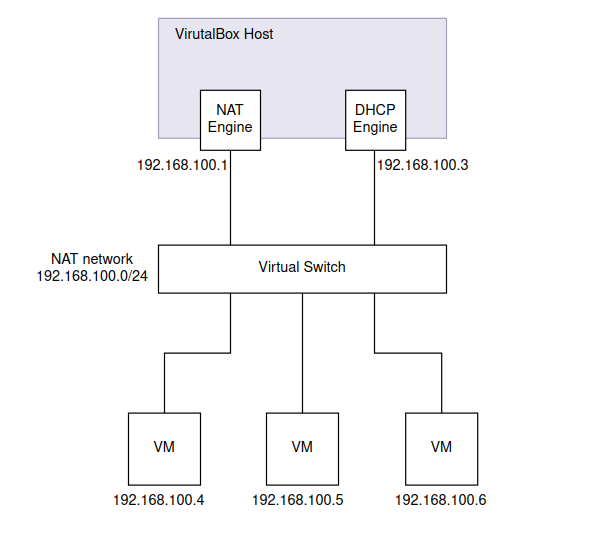
\includegraphics[width=0.5\textwidth]{dev.png}
\caption{Development Enviornment Architecture}
\label{fig:sandbox}
\end{figure}


\section{Deployment}

After achieving and configuring the prototype previously developed, the next phase focuses on the deployment of the solution within \ac{ua}'s premises. As already mentioned, the Headscale instance should be hosted in a server residing in \ac{ua}'s public domain segment. This allows the control server to be reachable to any client within the campus. Here, the configuration should be based on the research done during the previous phase, with few eventual changes to ports and/or addresses. Regarding clients, ideally, each team of robots should have its own user, which individual robots will use for authentication. <TODO: COMO SERA O PROCESSO DE GERAR KEYS???>.

Hence, this phase aims to (i) deploy an Headscale server in \ac{ua}'s public network domain, (ii) configure robots to act as Tailscale clients and (iii) establish communication within a team of robots spread out throughout the campus.


\section{Automation}
\label{sec:automethod}

This final development phase aims to create automation processes to aid in the deployment and configuration of the solution.

So, the automation process has two main goals in mind: First, to (i) provide a minimal configuration script to install and deploy an Headscale instance and provision its respective resources (auth keys, users, \acp{acl}) and (ii) provide a script installing Tailscale's client and configuring the system to automatically join the desired network.

\section{Work Plan}

The tasks encompassing the phases described above can be summed up in a Gantt diagram, presented in figure \ref{fig:gantt}. The tasks to be carried out are as follows:

\begin{itemize}
  \item \textbf{Development Environment Design and Requirement Analysis} - Setup of the development environment and minimum requirement analysis (identification of packets, accounts creation and domain definitions)
  \item \textbf{Prototype Development} - Implementation, in the development environment, of a prototype fulfilling the requirements. The end goal is to establish a \ac{p2p} connection between the two machines that can't communicate.
  \item \textbf{Deployment} - Deployment of the control server in \ac{ua}'s public services domain and configuration of clients in the robots.
  \item \textbf{Validation} - Validation of the deployed solution, ensuring encrypted communication between nodes in different geographical locations within the campus.
  \item \textbf{Automation} - Development of config-based scripts automating client and server configurations.
  \item \textbf{Final Document Writing} - Writing of the final document, presenting the development process and providing analysis of respective results.
\end{itemize}

\begin{figure}[h]
\centering
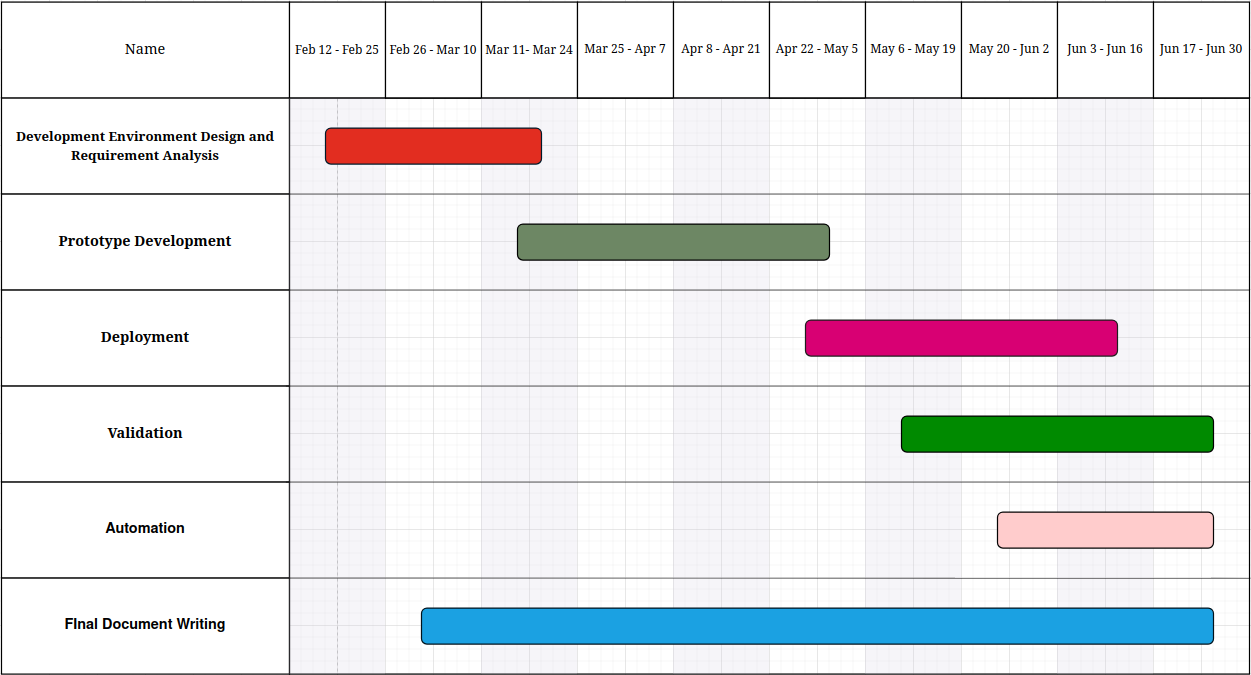
\includegraphics[width=1\textwidth]{gantt.png}
\caption{Development planning proposal}
\label{fig:gantt}
\end{figure}

\chapter{Prototype Development}

This chapter details the configuration of the development environment, as proposed in figure \ref{fig:sandbox}, and its use for the implementation of a prototype. This environment is managed with Oracle Virtual Box. Having defined the goals for this experiment in the aforestated work porposal, this prototype requires the deployment of the Headscale control server, which is hosted in \textbf{VM-3}, followed by the configuration, and respective authentication of both clients, \textbf{VM-1} and \textbf{VM-2}, using the Tailscale \ac{cli}. With the clients configured with Tailscale addresses, these can be used to run tests on \ac{ros} applications.

\section{Development Environment}

\subsubsection{Virtual Machines}

The three virtual machines composing the environment use \emph{Ubuntu Server 22.04} as their operating system. Due to the nature of the goals to be achieved in this phase, which focus on an extremly narrow scope, the machines require very little resources. Regarding networking, \textbf{VM-3} is attached to a bridge network on the ethernet interface of the host machine. As for \textbf{VM-1} and \textbf{VM-2}, each respective network adapter is attached to a \ac{nat}, isolating each client on its own private network, unaccessible from the outside. All machines can access the internet through the access point, explored in the following subsection.

Both \textbf{VM-1} and \textbf{VM-2} are assigned the same private \ac{ip} address since they are residing in distinct private networks. For convenience, the Virtual Machines are also configured to allow \ac{ssh} connections, which means port 22 is open on all machines. Moreover, for machines \textbf{VM-1} and \textbf{VM-2}, which are confined to their private networks, this was achieved with port forwarding rules, forwarding \textbf{VM-1}'s port 22 to the host machine's port 2222 and \textbf{VM-2}'s port 22 to the host machine's port 2223.

Table \ref{table:vmspecs} summarizes said specification.

\begin{table}[]
\centering
\resizebox{\textwidth}{!}{
     \begin{tabular}{c|c|c|c|c|}
     \cline{2-4}
     \multicolumn{1}{l|}{}                           & \textbf{VM-1}        & \textbf{VM-2}        & \textbf{VM-3}        \\ \hline
     \multicolumn{1}{|c|}{\textbf{Operating System}} & Ubuntu Server 22.04 & Ubuntu Server 22.04 & Ubuntu Server 22.04 \\ \hline
     \multicolumn{1}{|c|}{\textbf{Memory (Mb)}}      & 1024                & 1024                & 1024                \\ \hline
     \multicolumn{1}{|c|}{\textbf{Storage (Gb)}}     & 10                  & 10                  & 10                  \\ \hline
     \multicolumn{1}{|c|}{\textbf{CPUs}}             & 1                   & 1                   & 1                   \\ \hline
     \multicolumn{1}{|c|}{\textbf{Network Adapter}}  & NAT                 & NAT                 & Bridged (ethernet)  \\ \hline
     \multicolumn{1}{|c|}{\textbf{Address}}          & 10.0.2.15           & 10.0.2.15           & 192.168.10.214      \\ \hline
     \end{tabular}
}
\caption{Development Virtual Machines specification}
\label{table:vmspecs}
\end{table}

\subsubsection{Access Point}

The access point used in this environment is a N600 Wireless Dual Band Gigabit router. The host machine is connected to the access point via ethernet. With this setup, when one of the client machines wants to communicate with \textbf{VM-3}, the traffic will be routed from the client to the \ac{ap}'s Wi-Fi interface. Then the router will forward the packet through its ethernet interface, reaching the host machine and, consequently, reaching \textbf{VM-3}, as its network adapter is bridged to the host's ethernet interface, as described above.

\section{Headscale Instance Deployment}
\label{sec:devhs}

Headscale provides an highly configurable open-source implementation of a control server, allowing the configuration of \ac{DERP} relays and \ac{stun} servers, which must also be hosted in this server. At the time of writing, the latest stable Headscale release is \emph{v0.22.3} \footnote{Headscale's official releases, hosted in GitHub. https://github.com/juanfont/headscale/releases.}, which is the version of the software refered to in the rest of this chapter.

The instance was configured to run with an embedded \ac{DERP} server in a sample region, which additionally provides \ac{stun} functionalities to make \ac{nat} traversal possible within the environment. These configurations were achieved through Headscale's configuration file, a yaml provided in the package. With the service running, \textbf{VM-3} is now listening for Tailscale clients to connect and start using the protocol. For development purposes, an Headscale user, \textbf{dev}, was registred in the instance and shall be the user the clients will register themselves with. Finally, regarding Tailscale \ac{ip} assignments, the instance uses the default subnet prefixes, 100.64.0.0/10 for ipv4 and fd7a:115c:a1e0::/48 for ipv6. Registered clients will be assigned \ac{ip} addresses in these ranges.

Table \ref{table:hstest} presents the available services and their respective listening configuration produced by the running Headscale instance. Besides the metrics and gRPC services, which are not required by clients to use the Tailscale protocol, are listening privately, on the server's localhost interface. The remaining services are exposed in the defined ports, reachable by the clients.

\begin{table}[]
\centering
\resizebox{\textwidth}{!}{
     \begin{tabular}{|c|c|c|c|}
     \hline
     \textbf{Service}                                                 & \textbf{Listen Address} & \textbf{Port} & \textbf{Description}                                         \\ \hline
     Control Server                                                   & 192.168.10.214          & 8080          & Main service implementing the control plane \\ \hline
     Metrics                                                          & 127.0.0.1               & 9090          & Exposes the /metrics endpoints, for monitoring               \\ \hline
     \end{tabular}
}
\caption{Services running in the Headscale instance}
\label{table:hstest}
\end{table}


\section{Client Configuration}

Initially, clients can't really establish a direct connection in a traditional way. In fact, neither client is assigned a public address which could be used as a communication's endpoint, nor do tehy possess any information regarding one another. They can, however, reach the outside internet, which consequently implies the translation of their private addresses into public ones, a process carried by the adapter attached to the host machine's \ac{nat}. <TODO: explicar teoria de porque é que o tailscale vai funcionar aqui>

Using Tailscale's \ac{cli}, a client is able to authenticate in the Headscale instance previously deployed, which in turn configures its Tailscale interface with a respective Tailscale \ac{ip}, in the range previously configured in the control server. This will allow a state where \ac{p2p} WireGuard tunnels can be established freely between the registered clients.

Hence, the Tailscale binaries were installed in each client, using Tailscale's install shell script \footnote{Tailscale's install script, publicly available online. https://tailscale.com/install.sh}.

At this point, clients are ready to perform authentication in the control server and start communicating, a process described in the next section.

\section{Authentication}

Authenticating in the Headscale instance can be done either using a pre-authenticated key, generated by the control sever and shared with a client, or by accessing the instance through the browser in the client side. For automation purposes, the authentication keys provide a much more useful mechanism presenting itself as the option more adequate for this solution.

With that said, reusable keys were generated in the control server with Headscale's \textbf{headscale preauthkeys create}, an utility included in the software's \ac{cli}, and shared with its respective clients. Clients are now able to authenticate with Tailscale's \ac{cli}, by using the \textbf{tailscale up} command. Two additional command-line parameters are set, the \emph{login-server}, which points to the address Headscale is listening and the \emph{authkey}, where the previously shared pre-authenticated key is injected.

With the clients authenticated, both devices are respectively assigned a Tailscale IP and hostname, used to communicate through the overlay network. Table \ref{tab:tsips} presents the clients' Tailscale configurations at this state.

\begin{table}[]
\centering
\begin{tabular}{c|c|c|}
\cline{2-3}
\textbf{}                                         & \textbf{VM-1} & \textbf{VM-2} \\ \hline
\multicolumn{1}{|c|}{\textbf{Tailscale Hostname}} & dev-1         & dev-2         \\ \hline
\multicolumn{1}{|c|}{\textbf{Tailscale IP (v4)}}  & 100.64.0.1    & 100.64.0.2    \\ \hline
\multicolumn{1}{|c|}{\textbf{Tailscale IP (v6)}}  & fd7a:115c:a1e0::1     & fd7a:115c:a1e0::2         \\ \hline
\end{tabular}
\caption{Clients Tailscale configuration after authentication}
\label{tab:tsips}
\end{table}

\section{Communication with ROS}

With both clients up and communicating, our last validation in this environment aims to ensure the connections are compatible with the \ac{ros} middleware. Therefore, a very simple \ac{ros} scenario was deployed in the clients. As the scope for this experiment lies solely on validating communication through Tailscale in a \ac{ros} context, clients are only required to run a very basic \ac{ros} distribution, hence, a no-GUI package, \textbf{ros-noetic-ros-base} \footnote{ROS-Base (Bare Bones). Basic ROS packaging, build and communication libraries. No GUI. Pulled from public repositories.} was installed in both clients.

The experiment starts by configuring \textbf{VM-1} as a \ac{ros} Master, achieved with the \textbf{ros-core} command which automatically assigns the host as the new master, listening on port 11311, under the \textbf{ROS\_HOSTNAME} dev-1, matching its Tailscale hostname for convenience. Then, \textbf{VM-2} should acknowledge \textbf{VM-1} as the \ac{ros} master. The \textbf{ROS\_MASTER\_URI} environment variable points to where the \ac{ros} Master is listening. Hence, \textbf{VM-2} sets this variable with \textbf{VM-1}'s \ac{ros} \ac{uri}, which is composed by \textbf{VM-1}'s Tailscale hostname and the previously established \ac{ros} port.

\textbf{VM-2} successfully configures its \ac{ros} ecosystem with \textbf{VM-1} as its master, effectively validating the use of Tailscale tunnels in conjunction with \ac{ros}' middleware.

\section{Chapter Summary}

This chapter details a successful implementation of a minimal configuration prototype which simulates, in an analogous environment, the interactions between a self-hosted Headscale control server and its clients. In fact, the configured environment presented a situation where two nodes, due to their network topology, couldn't immediately establish a \ac{p2p} connection, but could both reach a third node. Headscale was then introduced in the public node as a self-hosted Tailscale control server, which, after authentication operations via pre-shared keys, made it possible to connect the client nodes through the Tailscale interfaces. Finally, this tunnel was tested when used along with \ac{ros}, operating as expected. The procedure taken in this phase meets the goals outlined in section \ref{sec:protodev}.

\chapter{Production Deployment}

The following chapter presents the configuration and deployment of a solution capable of being used by any client in the campus. As such, and as mentioned in previous sections, this implies that the Headscale instance must be available regardless of a client's physical location within the campus.

\section{Headscale Deployment}

In this solution, the Headscale instance is hosted within \ac{iris}'s network. This, however, only allows communications from clients residing in the \ac{iris}'s network. For clients to be able to reach the instance from any location in the campus, port forwarding rules were created on an exposed server in \ac{iris}'s network, accessible within \ac{ua}'s network, which redirects traffic on ports 8080 (the main Headscale service and the embedded \ac{DERP}) and 3478 (\ac{stun} interface) to the Headscale server. With this configuration, clients within the campus, which can directly reach the public facing proxy machine, can communicate with the Headscale instance. Figure \ref{fig:prodsolution} presents such architecture.

\begin{figure}[h]
\centering
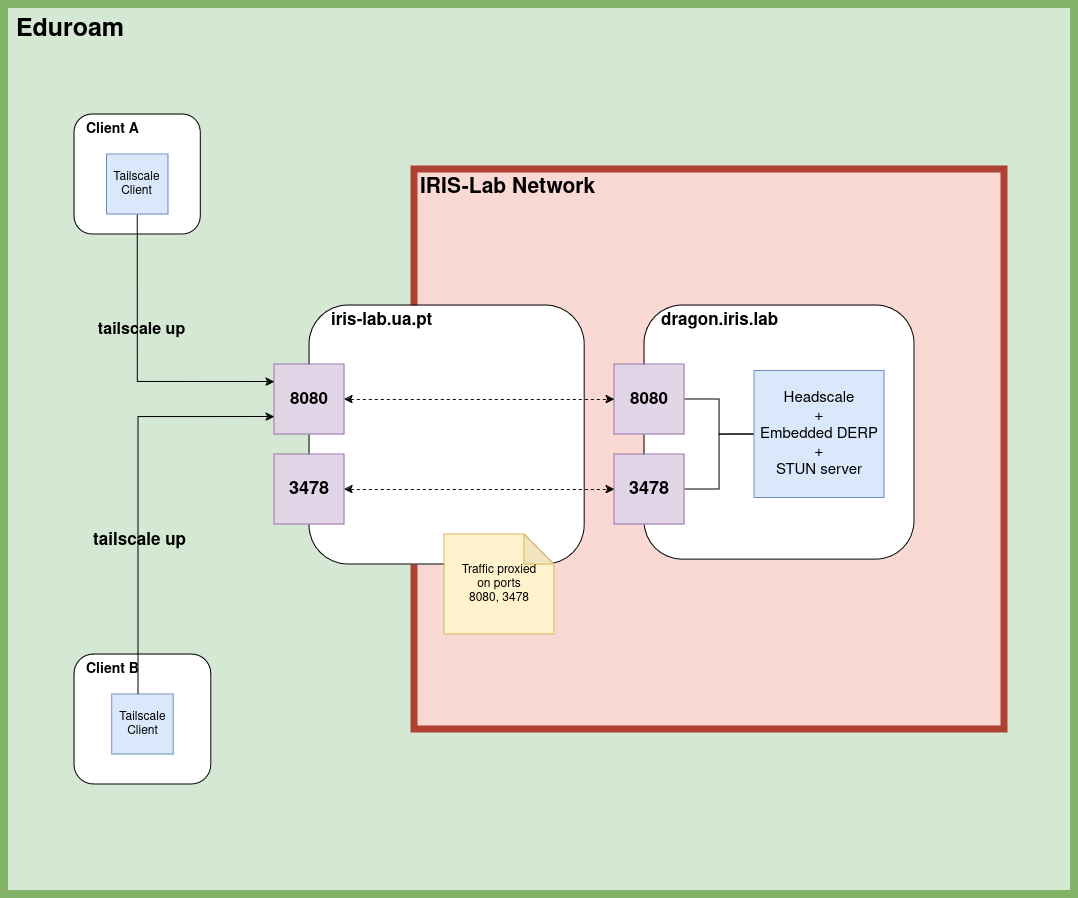
\includegraphics[width=\textwidth]{prod.png}
\caption{Production Deployment Architecture}
\label{fig:prodsolution}
\end{figure}

Since Headscale's host is also an Ubuntu linux environment, installation of this service followed the process described in the development environment (see Section \ref{sec:devhs}). Regarding configuration, however, the \textbf{server\_url} parameter, which points to the endpoint clients should use to authenticate, is now the \ac{fqdn} of the proxy server, \emph{iris-lab.ua.pt}.

\subsection{Self-Hosting DERP Infrastructure}

Initially, Headscale was configured to use Tailscale's \ac{DERP} server fleet. However, upon testing this scenario, established relayed connections, meaning \ac{DERP} servers are being used to redirect traffic over \ac{http}, implied the redirection of traffic to a \ac{DERP} server in Germany, resulting in tunnels with an average latency of 452ms, a value unacceptable for the scope of this dissertation. Moreover, as this solution is meant to be used exclusevly by \ac{ua}'s clients, traffic should be contained within the campus' network. Therefore, Tailscale's \ac{DERP} fleet was discarded, opting for a self-hosted alternative.

Headscale allows the use of an embedded \ac{DERP} server, which also exposes \ac{stun} functionalities for \ac{nat}-Traversal. This server can be enabled through Headscale's configuration file, and runs alongside Headscale's main service, on the same address and port. As for the \ac{stun} endpoints, these are also configured to run in the same address, on \ac{udp} port 3478.

Using the embedded self-hosted \ac{DERP} allows relayed communication between clients to be much more efficient, with much more appealing latencies (discussed in Chapter \ref{chap:results}).


\subsection{Adding server certificates}

To use the self-hosted \ac{DERP} server, Headscale is required to be exposed on an \ac{https} server, hence it needs a valid X509 certificate. Although Headscale's configuration allows a seamless integration with certificating tools such as \ac{le} or Caddy, in this scenario, where Headscale's \ac{fqdn} is not public, such methods can't be used. Alas, to certify Headscale, self-signed certificates were generated using the \textbf{openssl} \ac{cli} and added manually to the instance, by pointing to both certificate and key file paths through Headscale's configuration file. TODO: JUSTIFICAR PORQUE É QUE NAO HA ATTACK VECTOR.

Using self-signed certificates requires additional client certificate trust configurations, which shall be covered in the following section.

\section{Client Deployment}

\subsection{Tailscale and Self-Signed Certificates}
\label{sec:selfscale}

Tailscale's client does not support the use of self-signed certificates, even if the system trusts the certificate. Figure \ref{fig:tscert} presents the logic behind Tailscale's certificate validation. However, as an open-source codebase, this code can be freely modified and the binaries rebuilt to suit one's needs. Therefore, a fork of Tailscale was created, which shall be refered to as selfscale \footnote{selfscale's repository: https://github.com/VascoRegal/selfscale}.

selfscale implements a new command-line option, --\emph{allow-self-signed}, which stores a boolean value. When true, the certificate validation method allows the use of self-signed certificates.

With the use of this option, a self-signed certificate needs only to be trusted by the system to be valid in the eyes of Tailscale's client. Hence, this solution requires clients to run the binaries generated from selfscale's source code.

\begin{figure}
\centering
\begin{lstlisting}
conf.VerifyConnection = func(cs tls.ConnectionState) error {
     // Perform some health checks on this certificate before we do
     // any verification.
     if ht != nil {
          if certIsSelfSigned(cs.PeerCertificates[0]) {
               // Self-signed certs are never valid.
               ht.SetTLSConnectionError(
                    cs.ServerName,
                    fmt.Errorf("certificate is self-signed")
               )

          } else {
               // Ensure we clear any error state for
               // this ServerName.
               ht.SetTLSConnectionError(cs.ServerName, nil)
          }
     }
     ...
\end{lstlisting}
\label{fig:tscert}
\caption{Snippet from Tailscale's client certificate verification method. Self-signed certificates are always considered invalid. /net/tlsdial/tlsdial.go, lines 79-90 }
\end{figure}

\subsection{Trusting Headscale}

As the Tailscale client can now accept self-signed certificates, Headscale's certificate can be added to the client machine's trusted list. On debian distributions, this required moving the certificate to the \emph{/usr/local/share/ca-certificates} and updating the list with the command \textbf{update-ca-certificates}. Installation scripts are available on a public repository.

\chapter{Automation}

This chapter details the development of automation tools to speed up deployment and configuration processes. In Section \ref{sec:automethod}, two main goals were defined, related to automatic deployments of the control server and clients. First, automating the deployment of a configured Headscale instance. This implies automating software installation, configuration applying and certificate management. Regarding clients, deployments require the installation of the custom binaries, explored in Section \ref{sec:selfscale}, adding Headscale's certificate to the trust list and, finally, authenticate to a desired network.

\section{Distributing Selfscale binaries}

Tailscale's codebase provides a script to build the binaries, which is also used to build Selfscale. Additionally, a configuration file is provided to setup Tailscale's daemon as a service.

Regarding distribution, these are hosted as a compressed file in the GitHub repository. TODO: Distributing the software as a package would probably be more optimal.

To generate the compressed package, a shell script was developed, \textbf{build\_selfscale.sh}, which builds both the tailscale and tailscale daemon binaries and zips them with the aforementioned configuration file. This zip is hosted on the \textbf{selfscale} folder of the repository. Currently this script is used to release a new version.

\section{Headscale Deployment}

Headscale's deployment requires both the installation of the software and its configuration, namely the configuration yaml and the server certificate. These last files are publicly available in the automation repository \footnote{Project automation repository, publicly available. https://github.com/VascoRegal/ua-overlays-automation}.

Hence, the \textbf{install\_headscale.sh} shell script starts by downloading a desired Headscale package, where version and system architecutre are specified with command-line arguments. Then, the script fetches the Headscale's configuration yaml, publicly available in the automation repository, and applies it to the instance. Finally, a x509 self-signed certificate is generated with the \textbf{openssl} \ac{cli} and placed, along with the certificate's key, in its respective path (matching what was defined in the the yaml).

\section{Client Deployment}

A shell script was also created for the clients. Here, configuring a client requires the installation of the modified Tailscale bianries, which can be downloaded as a zip from Selfscale's GitHub repository. Then, the package is extracted and files are placed accordingly. Then, Headscale's server certificate is also fetched and added to the system's trust mechanisms. 

Running this simple script leaves a machine in a state where, given a pre-shared key, authentication can be performed with the \textbf{tailscale up} command.

\chapter{Validation and Results}
\label{chap:results}

To validate the solution, two dimensions must be taken into account. First, it is necessary to ensure clients can use the overlay networks from anywhere within the campus. Then, the overall network performance should also be analyzed, namely communication latencies, network throughput both for \ac{tcp} and \ac{udp} and network jitter. Fortunatelly, both scopes can be tested simultaneously!

\textbf{iperf3} is an open-source tool which measures several of such metrics by exchanging packets on a client-server model. Regarding latencies, these can be measured with simple \textbf{ping} commands.

Therefore, these tests were implemented as a python script \footnote{https://github.com/VascoRegal/ua-overlays-automation/blob/main/tests/network/iperf/analysis.py} which connects to a host to run \textbf{iper3} \ac{tcp} and \ac{udp} tests for 120 seconds each and exporting the results as \ac{json}. To this \ac{json} is added the average latency by executing the \textbf{ping} command with a limit of 50 replies.

For this experiment, a Tailscale client running \textbf{iper3} as a server was placed inside \ac{iris} network. Then, with another machine, the script was run in clients connected to \ac{ua}'s network, from disperse points in the campus. This procedure allows not only the collection of \textbf{iperf3}'s network metrics and latencies but also the validation of the solution's coverage, since the script connects to the \ac{iris}'s host with its Tailscale IP. If this connection fails, Tailscale can't cover that area, possibly due to more constraining networking rules. As it will be shown in the following sections, however, none of the tested areas failed to establish communication.

\section{Campus Coverage}

For coverage testing, twelve different scenarios were considered, presented on table \ref{tab:locs}.

\begin{table}[]
  \centering
\begin{tabular}{|c|c|c|}
\hline
\textbf{Location}                                                                                             & \textbf{\begin{tabular}[c]{@{}c@{}}Building\\ ID\end{tabular}} & \textbf{\begin{tabular}[c]{@{}c@{}}Connection\\ Type\end{tabular}}     \\ \hline
\begin{tabular}[c]{@{}c@{}}IRIS-Lab\\ (IRIS)\end{tabular}                                                     & 19                                                                 & Internal                                                               \\ \hline
\begin{tabular}[c]{@{}c@{}}IRIS-Lab\\ (IRIS)\end{tabular}                                                     & 19                                                                 & \begin{tabular}[c]{@{}c@{}}Tailscale\\ (direct)\end{tabular}  \\ \hline
\begin{tabular}[c]{@{}c@{}}University Library\\ (BIB)\end{tabular}                                          & 17                                                                 & \begin{tabular}[c]{@{}c@{}}Tailscale\\ (relayed)\end{tabular} \\ \hline
\begin{tabular}[c]{@{}c@{}}Political Science Department\\ (DSCPT)\end{tabular}                              & 12                                                                 & \begin{tabular}[c]{@{}c@{}}Tailscale\\ (relayed)\end{tabular} \\ \hline
\begin{tabular}[c]{@{}c@{}}Communication and Arts Department\\ (DECA)\end{tabular}                          & 21                                                                 & \begin{tabular}[c]{@{}c@{}}Tailscale\\ (relayed)\end{tabular} \\ \hline
\begin{tabular}[c]{@{}c@{}}Student's Bar\\ (BE)\end{tabular}                                                  & N                                                                  & \begin{tabular}[c]{@{}c@{}}Tailscale\\ (relayed)\end{tabular} \\ \hline
\begin{tabular}[c]{@{}c@{}}Eletronics, Telecomunications and Informatics\\ Department\\ (DETI)\end{tabular} & 4                                                                  & \begin{tabular}[c]{@{}c@{}}Tailscale\\ (relayed)\end{tabular} \\ \hline
\begin{tabular}[c]{@{}c@{}}Exhibition Hall\\ (EXPO)\end{tabular}                                              & 24                                                                 & \begin{tabular}[c]{@{}c@{}}Tailscale\\ (relayed)\end{tabular} \\ \hline
\begin{tabular}[c]{@{}c@{}}Pedagogical Complex\\ (CP)\end{tabular}                                            & 23                                                                 & \begin{tabular}[c]{@{}c@{}}Tailscale\\ (relayed)\end{tabular} \\ \hline
\begin{tabular}[c]{@{}c@{}}Mathematics Department\\ (DMAT)\end{tabular}                                     & 11                                                                 & \begin{tabular}[c]{@{}c@{}}Tailscale\\ (relayed)\end{tabular} \\ \hline
\begin{tabular}[c]{@{}c@{}}Biology Department\\ (DBIO)\end{tabular}                                         & 8                                                                  & \begin{tabular}[c]{@{}c@{}}Tailscale\\ (relayed)\end{tabular} \\ \hline
\begin{tabular}[c]{@{}c@{}}Economics and Management Department\\ (DEGEIT)\end{tabular}                      & 10                                                                 & \begin{tabular}[c]{@{}c@{}}Tailscale\\ (relayed)\end{tabular} \\ \hline
\end{tabular}
\caption{Locations and scenarios used for validation}
\label{tab:locs}
\end{table}

\section{Network Performance}

\subsection{Throughput}

\subsubsection{TCP}

\begin{figure}[h]
\centering
  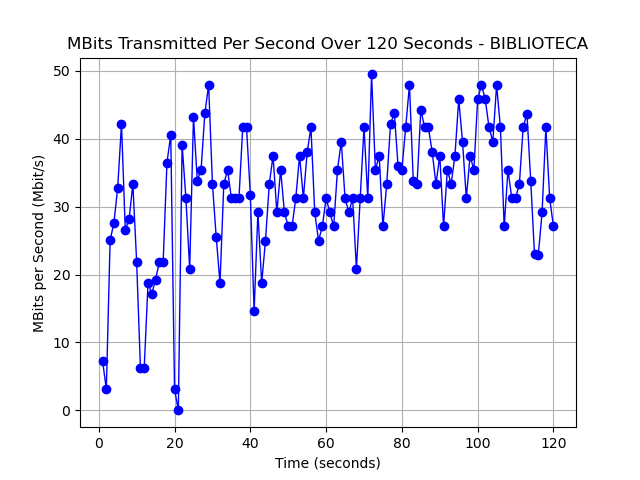
\includegraphics[width=0.8\textwidth]{biblioteca-tcp.png}
  \caption{TCP Tailscale tunnel Network TCP Throughput (University Library)}
  \label{fig:tcptplibrary}
\end{figure}

\subsubsection{UDP}

\begin{figure}[h]
\centering
  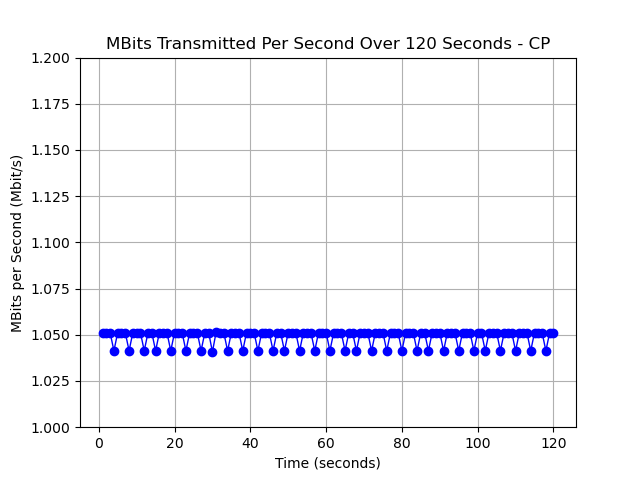
\includegraphics[width=0.8\textwidth]{cp-udp.png}
  \caption{UDP Tailscale tunnel Network Throughput (Pedagogic Complex)}
  \label{fig:tcptplibrary}
\end{figure}

\subsection{Latency}

\begin{figure}[h]
\centering
  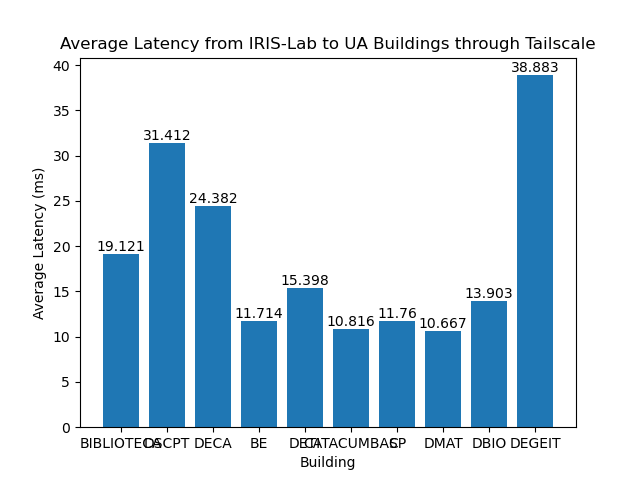
\includegraphics[width=0.8\textwidth]{building-latency.png}
  \caption{Average latencies by campus location}
  \label{fig:udptpcp}
\end{figure}


\begin{figure}[h]
\centering
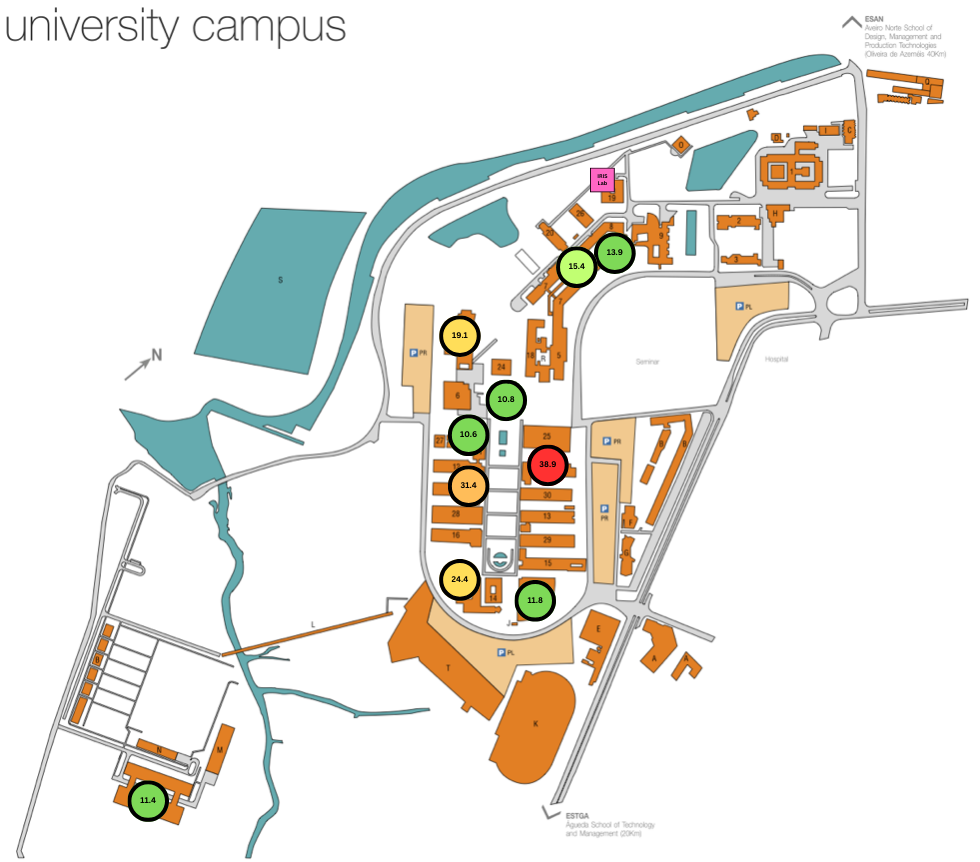
\includegraphics[width=0.8\textwidth]{ua-latency.png}
\caption{Average latency on a Tailscale connection from different UA buildings to IRIS-Lab. The numbers in the circles represent average latency values.}
\label{fig:ualats}
\end{figure}


\subsection{Jitter}

\begin{figure}[h]
\centering
  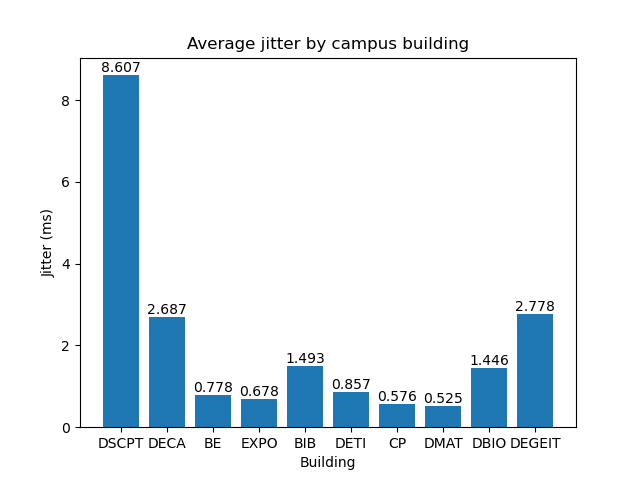
\includegraphics[width=0.8\textwidth]{building-jitter.png}
  \caption{Network Jitter by campus location.}
  \label{fig:uajitter}
\end{figure}

\chapter{Conclusion}


%
% The bibliography
%
\cleardoublepage
\iffalse
  % Use this is the final version
  %  unsrt produces numbered entries, sorted by order of citation
  %  plain produces numbered entries, sorted alphabetically
  %  other styles are possible (I recommend the harvard package)
  %\bibliographystyle{ieeetr}
  \bibliography{my-bib-file}% replace by the name of name of your .bib file
\else
  % An example (the contents of the .bbl file)
  %\begin{thebibliography}{10}



  %\end{thebibliography}
%\fi

\bibliographystyle{ieeetr}
\bibliography{refs}
\cleardoublepage

\end{document}
